\documentclass[conference]{IEEEtran}
\IEEEoverridecommandlockouts
\usepackage{cite}
\usepackage{amsmath,amssymb,amsfonts}
\usepackage{algorithmic}
\usepackage{graphicx}
\usepackage{textcomp}
\usepackage{xcolor}
\usepackage{booktabs}
\usepackage{multirow}
\usepackage{subcaption}
\usepackage{tikz}
\usetikzlibrary{arrows.meta, positioning, calc, decorations.pathreplacing, shapes.geometric, fit, backgrounds, patterns}
\def\BibTeX{{\rm B\kern-.05em{\sc i\kern-.025em b}\kern-.08em
    T\kern-.1667em\lower.7ex\hbox{E}\kern-.125emX}}

\begin{document}

\title{Empirical Characterization of Network Delay Variability Relevant to Real-Time Multiplayer Game Traffic}

\author{\IEEEauthorblockN{Anonymous Author(s)}
}

\maketitle

\begin{abstract}
Real-time multiplayer games depend on low and predictable network latency for responsiveness and competitive fairness. While delay compensation techniques are well studied, the empirical delay distributions that underpin their design assumptions remain less systematically characterized across geographic scales. This paper presents a measurement-driven characterization of round-trip time (RTT) variability across 36 Internet paths spanning three distance regimes: short-haul (under 500\,km), regional (1\,000 to 2\,200\,km), and intercontinental (5\,500 to 17\,500\,km). Using active probes from the RIPE Atlas anchor mesh over a 14-day observation window, we collect 181\,440 RTT samples across ICMP, UDP, and TCP protocols and fit candidate distributions. All 36 paths are best described by the log-normal distribution under both Kolmogorov-Smirnov testing and Bayesian information criterion selection. We confirm statistically significant diurnal patterns across all paths ($p < 0.05$) and strong regime separation (Kruskal-Wallis $H = 160{,}913$, $p < 0.001$). Cross-validation against 41\,655 passive TCP SYN-ACK samples from MAWI and 5\,577 traceroute-derived samples from CAIDA Ark confirms distributional consistency across three independent measurement methodologies. Multi-protocol comparison shows maximum per-regime delay differences of 20.7\% between ICMP and TCP. From the measured data, we derive a five-level empirical delay taxonomy and compare it against profiles used in a prior delay equalization study, finding those assumed profiles to be 34 to 63\% more conservative than empirical measurements. We map each taxonomy level to latency tolerance thresholds for six game genres, providing practitioners with empirically grounded guidance for delay model selection and server placement.
\end{abstract}

\begin{IEEEkeywords}
network delay, round-trip time, latency characterization, multiplayer games, RIPE Atlas, CAIDA, measurement study, delay distribution
\end{IEEEkeywords}

%% ===================================================================
%%  SECTION I -- INTRODUCTION
%% ===================================================================
\section{Introduction}

The timely delivery of messages between clients and servers is central to online multiplayer games and other latency-sensitive distributed systems. In such environments, fairness and responsiveness depend on participants receiving information and having their actions processed under comparable network conditions. Differences in network delay create information asymmetries that favor clients with lower latency: server state updates reach nearby clients sooner, while actions from distant clients arrive later. Consequently, participants with higher latency are disadvantaged both when receiving information and when responding to it.

Considerable research has addressed delay compensation at the client side (prediction and interpolation~\cite{bernier2001}), the server side (lag compensation and hit registration rewinding), and the network level (artificial delay injection for fairness~\cite{brun2006}, bucket synchronization~\cite{cronin2004}). These mechanisms rely, implicitly or explicitly, on assumptions about the statistical properties of the delays they seek to compensate. However, the empirical distributions, temporal structure, and geographic scaling of Internet round-trip times are not always systematically validated against the profiles used in system design and simulation.

Measurement studies have established that Internet delays exhibit right-skewed distributions, temporal autocorrelation, and diurnal variation~\cite{paxson1999}. Residential broadband characterizations~\cite{dischinger2007, sundaresan2011} have documented access-network delay behavior in detail. Yet few studies directly connect these measurement findings to the delay models used in game networking research, where simulation parameters are often drawn from rough estimates or legacy measurements rather than current empirical data. This gap between measurement science and system evaluation creates a risk: compensation mechanisms may be validated under conditions that do not reflect the delay environments in which they will operate.

This paper addresses that gap through a structured empirical characterization. We collect active RTT measurements from the RIPE Atlas anchor mesh~\cite{ripeatlas} across 36 paths spanning three distance regimes, cross-validate against passive TCP SYN-ACK timing data from the MAWI Working Group archive~\cite{mawi} and traceroute-derived RTTs from the CAIDA Ark infrastructure~\cite{caida}, and compare delay behavior across ICMP, UDP, and TCP protocols. From the measurements, we derive an empirical delay taxonomy and compare it against the profiles assumed in a prior delay equalization study~\cite{companion}. The contributions of this paper are:

\begin{enumerate}
\item A systematic RTT characterization across 36 Internet paths grouped into three distance regimes over a 14-day window, with distribution fitting, temporal analysis, and inter-regime significance testing.
\item Three-source cross-validation between active RIPE Atlas ICMP probes, passive MAWI TCP SYN-ACK timing, and CAIDA Ark traceroute-derived RTTs, confirming distributional consistency across independent measurement methodologies.
\item Multi-protocol comparison of ICMP, UDP, and TCP probes across all paths, quantifying protocol-dependent delay differences.
\item A five-level empirical delay taxonomy with quantitative comparison against assumed profiles from a prior equalization study, showing 34 to 63\% conservatism in those assumptions.
\item Mapping of empirical delay profiles to published latency tolerance thresholds for six game genres, yielding concrete server placement guidance.
\end{enumerate}

The remainder of this paper is organized as follows. Section~II surveys related work. Section~III describes the measurement methodology. Section~IV presents the statistical analysis results. Section~V derives the empirical taxonomy and assesses game relevance. Section~VI discusses implications and limitations. Section~VII concludes.

%% ===================================================================
%%  SECTION II -- RELATED WORK
%% ===================================================================
\section{Related Work}

\subsection{Internet Delay Measurement}

Paxson~\cite{paxson1999} provided one of the earliest large-scale characterizations of end-to-end Internet packet dynamics, documenting heavy-tailed delay distributions and significant path asymmetry. That work established the log-normal and related heavy-tailed models as canonical descriptions of Internet delay. Dischinger et~al.~\cite{dischinger2007} characterized residential broadband networks, measuring last-mile delay contributions across DSL, cable, and fiber access technologies. Sundaresan et~al.~\cite{sundaresan2011} extended this to gateway-level measurements, establishing that access-network variability dominates end-to-end delay for many paths.

The RIPE Atlas platform~\cite{ripeatlas} provides a globally distributed measurement infrastructure with thousands of probes and anchors. Bajpai et~al.~\cite{bajpai2015} documented lessons learned from using RIPE Atlas for measurement research. The MAWI Working Group maintains a public traffic archive from the WIDE backbone~\cite{mawi, cho2000}, from which passive RTT estimates can be extracted through TCP SYN-ACK timing analysis. Fontugne et~al.~\cite{fontugne2010} developed the MAWILab framework for anomaly detection on the same traces. The CAIDA Ark measurement infrastructure~\cite{caida} provides active traceroute measurements from globally distributed vantage points, enabling independent RTT estimation through router-level path tracing.

\subsection{Passive RTT Estimation}

TCP SYN-ACK timing provides a passive method for RTT estimation from packet captures without requiring cooperation from endpoints. Jiang and Dovrolis~\cite{jiang2002} formalized this approach, demonstrating that matching SYN and SYN-ACK packets yields RTT estimates with accuracy comparable to active probing. Moon et~al.~\cite{moon2000} addressed clock skew removal from network delay measurements, a technique that underpins both active and passive timing approaches.

\subsection{Delay in Game Networking}

Claypool and Claypool~\cite{claypool2006} provided a comprehensive taxonomy of latency effects across game genres, establishing empirical thresholds for perceptible and disruptive delay. Dick et~al.~\cite{dick2005} further quantified how delay differences of 50 to 80\,ms can shift competitive outcomes. Bernier~\cite{bernier2001} described entity interpolation and lag compensation techniques. Cronin et~al.~\cite{cronin2004} proposed bucket synchronization for mirrored architectures. Brun et~al.~\cite{brun2006} introduced artificial delay injection for peer-to-peer fairness. Adaptive playout mechanisms for packetized audio~\cite{ramjee1994}, while developed for VoIP, employ similar statistical delay modeling and have influenced jitter buffer design in game networking.

%% ===================================================================
%%  SECTION III -- MEASUREMENT METHODOLOGY
%% ===================================================================
\section{Measurement Methodology}

\subsection{Measurement Architecture}

Fig.~\ref{fig:architecture} illustrates the measurement setup. We use the RIPE Atlas anchor mesh~\cite{ripeatlas} as the primary data source, selecting 36 bidirectional paths between anchor nodes distributed across 32 cities on six continents. Paths are grouped into three distance regimes based on great-circle propagation distance:

\begin{itemize}
\item \textbf{Short-haul} (under 500\,km): same-city or neighboring-city pairs, representing intra-metropolitan and short domestic paths.
\item \textbf{Regional} (1\,000 to 2\,200\,km): same-continent pairs, representing typical within-continent connectivity.
\item \textbf{Intercontinental} (5\,500 to 17\,500\,km): cross-continent pairs, representing trans-oceanic and long-haul paths.
\end{itemize}

Each regime contains 12 paths to ensure balanced statistical comparison. Two independent data sources provide cross-validation: TCP SYN-ACK RTT samples extracted from the MAWI Working Group traffic archive~\cite{mawi, cho2000}, which provides passive packet captures from the WIDE backbone link in Tokyo, and traceroute-derived RTT samples from the CAIDA Ark measurement infrastructure~\cite{caida}, which provides active measurements from eight globally distributed vantage points.

%% --- Measurement Architecture TikZ (full-width) ---
\begin{figure*}[t]
\centering
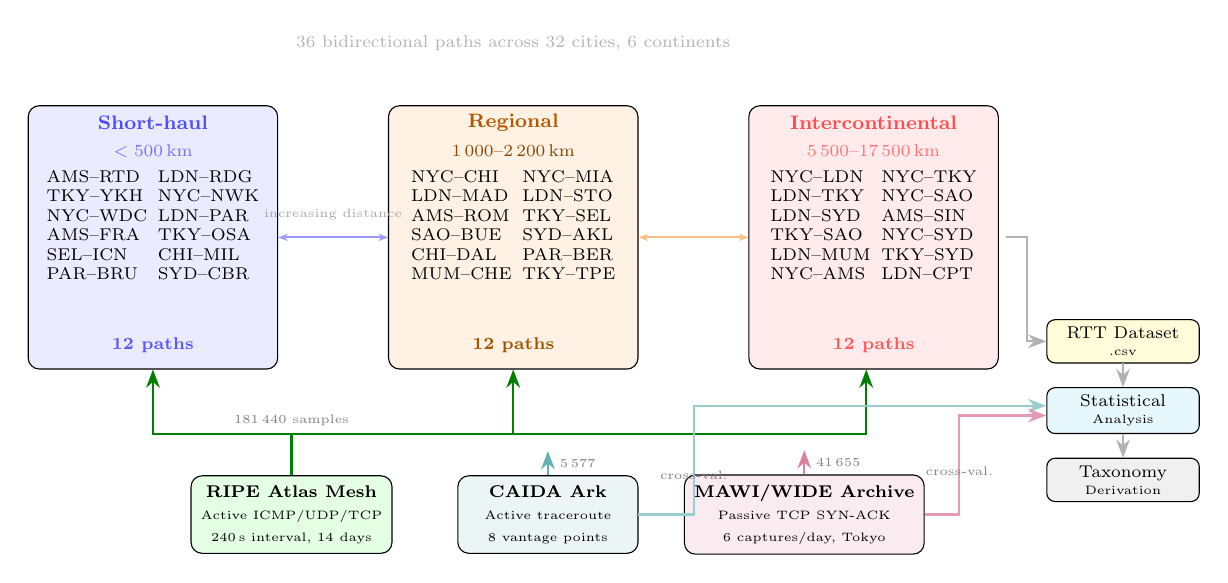
\begin{tikzpicture}[
    font=\small, >=Stealth,
    scale=0.88, every node/.style={scale=0.88},
    regionbox/.style={draw, rounded corners=4pt, fill=#1,
        minimum width=3.6cm, minimum height=3.8cm,
        inner sep=5pt, align=center},
    citynode/.style={font=\scriptsize, align=left},
    srcbox/.style={draw, rounded corners=4pt, fill=#1,
        minimum width=2.6cm, minimum height=1.1cm,
        inner sep=4pt, align=center},
    outbox/.style={draw, rounded corners=3pt, fill=#1,
        minimum width=2.2cm, minimum height=0.55cm,
        inner sep=3pt, align=center, font=\scriptsize},
    netcloud/.style={draw=gray!50, dashed, rounded corners=6pt,
        fill=gray!4, inner sep=5pt},
    pathlabel/.style={font=\scriptsize\itshape, align=center},
    biarrow/.style={{Stealth[length=3.5pt]}-{Stealth[length=3.5pt]}, thick},
    arr/.style={->, thick, gray!60},
]
%% ========== THREE REGIME BOXES ==========
%% Short-haul
\node[regionbox=blue!8] (sh) at (0, 0) {};
\node[font=\footnotesize\bfseries, text=blue!70] at (0, 1.65) {Short-haul};
\node[font=\scriptsize, text=blue!55] at (0, 1.25) {$< 500$\,km};
\node[citynode] at (0, 0.15) {%
\begin{tabular}{@{}l@{\;\;}l@{}}
AMS--RTD & LDN--RDG \\
TKY--YKH & NYC--NWK \\
NYC--WDC & LDN--PAR \\
AMS--FRA & TKY--OSA \\
SEL--ICN & CHI--MIL \\
PAR--BRU & SYD--CBR \\
\end{tabular}};
\node[font=\scriptsize\bfseries, text=blue!65] at (0, -1.55) {12 paths};

%% Regional
\node[regionbox=orange!10] (rg) at (5.2, 0) {};
\node[font=\footnotesize\bfseries, text=orange!70!black] at (5.2, 1.65) {Regional};
\node[font=\scriptsize, text=orange!55!black] at (5.2, 1.25) {1\,000--2\,200\,km};
\node[citynode] at (5.2, 0.15) {%
\begin{tabular}{@{}l@{\;\;}l@{}}
NYC--CHI & NYC--MIA \\
LDN--MAD & LDN--STO \\
AMS--ROM & TKY--SEL \\
SAO--BUE & SYD--AKL \\
CHI--DAL & PAR--BER \\
MUM--CHE & TKY--TPE \\
\end{tabular}};
\node[font=\scriptsize\bfseries, text=orange!65!black] at (5.2, -1.55) {12 paths};

%% Intercontinental
\node[regionbox=red!8] (ic) at (10.4, 0) {};
\node[font=\footnotesize\bfseries, text=red!70] at (10.4, 1.65) {Intercontinental};
\node[font=\scriptsize, text=red!55] at (10.4, 1.25) {5\,500--17\,500\,km};
\node[citynode] at (10.4, 0.15) {%
\begin{tabular}{@{}l@{\;\;}l@{}}
NYC--LDN & NYC--TKY \\
LDN--TKY & NYC--SAO \\
LDN--SYD & AMS--SIN \\
TKY--SAO & NYC--SYD \\
LDN--MUM & TKY--SYD \\
NYC--AMS & LDN--CPT \\
\end{tabular}};
\node[font=\scriptsize\bfseries, text=red!65] at (10.4, -1.55) {12 paths};

%% ========== REGIME CONNECTING PATHS ==========
\draw[biarrow, blue!40] (sh.east) -- (rg.west)
    node[midway, above=3pt, font=\tiny, gray!70] {increasing distance};
\draw[biarrow, orange!50] (rg.east) -- (ic.west)
    node[midway, above=3pt, font=\tiny, gray!70] {};

%% ========== DATA SOURCES (below) ==========
\node[srcbox=green!10] (ripe) at (2.0, -4.0) {%
\textbf{\scriptsize RIPE Atlas Mesh}\\[-2pt]
\tiny Active ICMP/UDP/TCP\\[-2pt]
\tiny 240\,s interval, 14 days};

\node[srcbox=teal!8] (caida) at (5.7, -4.0) {%
\textbf{\scriptsize CAIDA Ark}\\[-2pt]
\tiny Active traceroute\\[-2pt]
\tiny 8 vantage points};

\node[srcbox=purple!8] (mawi) at (9.4, -4.0) {%
\textbf{\scriptsize MAWI/WIDE Archive}\\[-2pt]
\tiny Passive TCP SYN-ACK\\[-2pt]
\tiny 6 captures/day, Tokyo};

%% ========== ARROWS FROM SOURCES TO REGIMES ==========
\draw[arr, green!50!black] (ripe.north) -- ++(0, 0.6) -| (sh.south);
\draw[arr, green!50!black] (ripe.north) -- ++(0, 0.6) -| (rg.south);
\draw[arr, green!50!black] (ripe.north) -- ++(0, 0.6) -| ([xshift=-3pt]ic.south);
\node[font=\tiny, gray, anchor=south] at (2.0,-2.85) {181\,440 samples};

\draw[arr, teal!60] (caida.north) -- ++(0, 0.35)
    node[pos=0.5, right=1pt, font=\tiny, gray] {5\,577};
\draw[arr, purple!50] (mawi.north) -- ++(0, 0.35)
    node[pos=0.5, right=1pt, font=\tiny, gray] {41\,655};

%% ========== OUTPUT (right) ==========
\node[outbox=yellow!15] (csv) at (14.0, -1.5) {RTT Dataset\\[-1pt]\tiny .csv};
\node[outbox=cyan!10] (anal) at (14.0, -2.5) {Statistical\\[-1pt]\tiny Analysis};
\node[outbox=gray!12] (tax) at (14.0, -3.5) {Taxonomy\\[-1pt]\tiny Derivation};

\draw[arr] ([xshift=3pt]ic.east) -- ++(0.3, 0) |- (csv.west);
\draw[arr] (csv.south) -- (anal.north);
\draw[arr] (anal.south) -- (tax.north);
\draw[arr, teal!40] (caida.east) -- ++(0.8, 0) |- ([yshift=2pt]anal.west)
    node[pos=0.12, above, font=\tiny, gray] {cross-val.};
\draw[arr, purple!40] (mawi.east) -- ++(0.5, 0) |- ([yshift=-2pt]anal.west)
    node[pos=0.15, above, font=\tiny, gray] {cross-val.};

%% ========== GLOBAL LABEL ==========
\node[font=\scriptsize, gray!60, align=center] at (5.2, 2.8)
    {36 bidirectional paths across 32 cities, 6 continents};
\end{tikzpicture}
\caption{Measurement architecture. Thirty-six paths between RIPE Atlas
anchors are grouped into three distance regimes. Active probes
(240\,s intervals over 14 days) yield 181\,440 ICMP RTT samples with
parallel UDP and TCP measurements.
MAWI passive TCP SYN-ACK captures (41\,655 samples) and CAIDA Ark
traceroute RTTs (5\,577 samples) provide independent cross-validation.}
\label{fig:architecture}
\end{figure*}

\subsection{Path Selection}

Table~\ref{tab:paths} lists the complete set of 36 measurement paths. Short-haul paths connect cities within the same metropolitan area or neighboring cities (e.g., Amsterdam to Rotterdam, 80\,km; Seoul to Incheon, 40\,km). Regional paths span distances within the same continent (e.g., New York to Chicago, 1\,150\,km; Mumbai to Chennai, 1\,340\,km). Intercontinental paths cross ocean boundaries (e.g., New York to Tokyo, 10\,850\,km; London to Cape Town, 9\,600\,km). The path set covers diverse geographic regions (North America, Europe, Asia, South America, Africa, Oceania) and a range of propagation distances within each regime.

%% --- Full 36-Path Table (full-width) ---
\begin{table*}[t]
\caption{Complete Measurement Path Set: 36 Paths Across Three Distance Regimes}
\label{tab:paths}
\begin{center}
\setlength{\tabcolsep}{3.5pt}
\begin{tabular}{clrcccc|clrcccc}
\toprule
\textbf{ID} & \textbf{Route} & \textbf{Dist.} & $\bar{d}$ & \textbf{Med.} & $\sigma$ & \textbf{Jit.} &
\textbf{ID} & \textbf{Route} & \textbf{Dist.} & $\bar{d}$ & \textbf{Med.} & $\sigma$ & \textbf{Jit.} \\
 & & (km) & (ms) & (ms) & (ms) & (ms) &
 & & (km) & (ms) & (ms) & (ms) & (ms) \\
\midrule
\multicolumn{7}{l}{\textit{Short-haul ($< 500$\,km)}} & \multicolumn{7}{l}{\textit{Regional (1\,000--2\,200\,km)}} \\
\cmidrule(lr){1-7} \cmidrule(lr){8-14}
sh\_01 & NYC--Newark & 25 & 7.9 & 7.9 & 1.3 & 1.0 &
rg\_01 & NYC--Chicago & 1\,150 & 32.0 & 31.7 & 5.0 & 4.1 \\
sh\_02 & LDN--Reading & 60 & 6.1 & 6.0 & 1.0 & 0.8 &
rg\_02 & NYC--Miami & 2\,000 & 45.5 & 45.1 & 7.2 & 6.0 \\
sh\_03 & AMS--Rotterdam & 80 & 5.0 & 5.0 & 0.8 & 0.7 &
rg\_03 & LDN--Madrid & 1\,260 & 38.2 & 37.8 & 6.5 & 5.3 \\
sh\_04 & TKY--Yokohama & 30 & 7.0 & 7.0 & 1.1 & 0.9 &
rg\_04 & LDN--Stockholm & 1\,430 & 42.7 & 42.2 & 6.6 & 5.6 \\
sh\_05 & NYC--Wash.\ DC & 360 & 12.1 & 11.9 & 2.2 & 1.8 &
rg\_05 & AMS--Rome & 1\,300 & 48.1 & 47.6 & 9.0 & 7.1 \\
sh\_06 & LDN--Paris & 340 & 14.3 & 14.1 & 2.7 & 2.2 &
rg\_06 & TKY--Seoul & 1\,160 & 35.5 & 35.0 & 6.5 & 4.9 \\
sh\_07 & AMS--Frankfurt & 365 & 11.1 & 11.0 & 1.9 & 1.5 &
rg\_07 & SAO--Buenos Aires & 1\,700 & 54.8 & 54.2 & 10.0 & 8.1 \\
sh\_08 & TKY--Osaka & 400 & 10.1 & 10.0 & 1.7 & 1.4 &
rg\_08 & SYD--Auckland & 2\,160 & 50.6 & 50.0 & 9.6 & 7.8 \\
sh\_09 & SEL--Incheon & 40 & 5.0 & 4.9 & 0.8 & 0.7 &
rg\_09 & CHI--Dallas & 1\,290 & 40.7 & 40.1 & 7.0 & 5.6 \\
sh\_10 & CHI--Milwaukee & 150 & 8.0 & 7.9 & 1.3 & 1.1 &
rg\_10 & PAR--Berlin & 1\,050 & 35.9 & 35.6 & 6.6 & 5.0 \\
sh\_11 & PAR--Brussels & 310 & 13.2 & 13.0 & 2.7 & 2.0 &
rg\_11 & MUM--Chennai & 1\,340 & 43.1 & 42.6 & 8.0 & 6.3 \\
sh\_12 & SYD--Canberra & 280 & 11.0 & 10.9 & 2.1 & 1.6 &
rg\_12 & TKY--Taipei & 2\,100 & 53.2 & 52.4 & 10.2 & 7.8 \\
\midrule
\multicolumn{14}{l}{\textit{Intercontinental (5\,500--17\,500\,km)}} \\
\cmidrule(lr){1-14}
ic\_01 & NYC--London & 5\,570 & 77.1 & 76.1 & 14.2 & 10.9 &
ic\_07 & TKY--S\~{a}o Paulo & 17\,500 & 264.7 & 261.7 & 41.8 & 34.3 \\
ic\_02 & NYC--Tokyo & 10\,850 & 173.0 & 171.1 & 25.3 & 21.1 &
ic\_08 & NYC--Sydney & 16\,000 & 252.8 & 250.3 & 35.2 & 29.4 \\
ic\_03 & LDN--Tokyo & 9\,560 & 233.7 & 231.2 & 35.0 & 27.7 &
ic\_09 & LDN--Mumbai & 7\,200 & 140.6 & 139.5 & 23.7 & 18.9 \\
ic\_04 & NYC--S\~{a}o Paulo & 7\,700 & 133.2 & 131.7 & 20.3 & 17.4 &
ic\_10 & TKY--Sydney & 7\,800 & 156.2 & 154.5 & 23.8 & 20.7 \\
ic\_05 & LDN--Sydney & 17\,000 & 273.3 & 270.5 & 38.0 & 31.5 &
ic\_11 & NYC--Amsterdam & 5\,850 & 84.0 & 83.0 & 13.6 & 11.3 \\
ic\_06 & AMS--Singapore & 10\,000 & 186.7 & 184.9 & 28.4 & 23.2 &
ic\_12 & LDN--Cape Town & 9\,600 & 196.2 & 194.3 & 29.7 & 24.0 \\
\bottomrule
\end{tabular}
\end{center}
\end{table*}

\subsection{Measurement Parameters}

RIPE Atlas ICMP ping measurements are collected at 240-second intervals over a continuous 14-day observation window, yielding 5\,040 samples per path and 181\,440 samples in total across all 36 paths. This interval balances measurement granularity against platform rate limits and captures diurnal, day-of-week, and longer-term temporal patterns. The 14-day window provides sufficient data for robust statistical analysis while remaining short enough to represent a coherent snapshot of network conditions.

To assess protocol-dependent delay differences, we collect parallel UDP and TCP probe measurements at the same 240-second interval across all 36 paths, yielding 181\,440 additional samples per protocol. This multi-protocol design enables quantification of any differential treatment of ICMP, UDP, and TCP traffic by network operators.

For the MAWI dataset, six 15-minute packet captures per day are processed at hours 02:00, 06:00, 10:00, 14:00, 18:00, and 22:00 JST, spanning the same 14-day window. TCP SYN-ACK pairs are matched to extract per-flow RTT estimates following the methodology of Jiang and Dovrolis~\cite{jiang2002}. This yields 41\,655 SYN-ACK RTT samples spanning domestic, regional, intercontinental, and satellite-served paths visible from the WIDE backbone. CAIDA Ark traceroute measurements from eight vantage points yield 5\,577 RTT samples derived from router-level round-trip timing.

\subsection{Analysis Pipeline}

Fig.~\ref{fig:pipeline} summarizes the analysis methodology. Raw RTT measurements pass through eight stages: (1)~per-path statistical characterization (moments, percentiles, autocorrelation, jitter metrics); (2)~distribution fitting against five candidate models (log-normal, gamma, Weibull, normal, Gumbel) with selection by BIC; (3)~temporal decomposition into hourly and daily patterns with ANOVA significance testing; (4)~inter-regime significance testing (Kruskal-Wallis, pairwise Mann-Whitney~U, distance-delay correlation); (5)~three-source cross-validation (RIPE Atlas vs. MAWI and CAIDA); (6)~multi-protocol comparison (ICMP vs. UDP vs. TCP); and (7)~taxonomy derivation with (8)~game relevance mapping.

%% --- Analysis Pipeline TikZ (single column) ---
\begin{figure}[t]
\centering
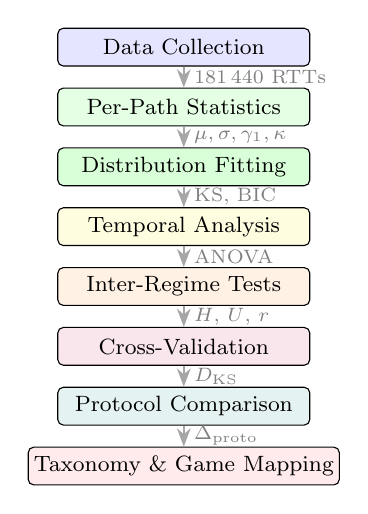
\begin{tikzpicture}[
    font=\footnotesize,
    >=Stealth,
    block/.style={draw, rounded corners=2pt, fill=#1,
        minimum width=3.2cm, minimum height=0.48cm,
        inner sep=2pt, align=center},
    arr/.style={->, thick, gray!70},
]
\node[block=blue!10]    (d1) at (0,  0)    {Data Collection};
\node[block=green!10]   (d2) at (0, -0.76) {Per-Path Statistics};
\node[block=green!15]   (d3) at (0, -1.52) {Distribution Fitting};
\node[block=yellow!12]  (d4) at (0, -2.28) {Temporal Analysis};
\node[block=orange!10]  (d5) at (0, -3.04) {Inter-Regime Tests};
\node[block=purple!10]  (d6) at (0, -3.80) {Cross-Validation};
\node[block=teal!10]    (d7) at (0, -4.56) {Protocol Comparison};
\node[block=red!8]      (d8) at (0, -5.32) {Taxonomy \& Game Mapping};
%% Arrows
\draw[arr] (d1) -- (d2) node[midway, right, font=\scriptsize, gray] {181\,440 RTTs};
\draw[arr] (d2) -- (d3) node[midway, right, font=\scriptsize, gray] {$\mu, \sigma, \gamma_1, \kappa$};
\draw[arr] (d3) -- (d4) node[midway, right, font=\scriptsize, gray] {KS, BIC};
\draw[arr] (d4) -- (d5) node[midway, right, font=\scriptsize, gray] {ANOVA};
\draw[arr] (d5) -- (d6) node[midway, right, font=\scriptsize, gray] {$H$, $U$, $r$};
\draw[arr] (d6) -- (d7) node[midway, right, font=\scriptsize, gray] {$D_{\text{KS}}$};
\draw[arr] (d7) -- (d8) node[midway, right, font=\scriptsize, gray] {$\Delta_{\text{proto}}$};
\end{tikzpicture}
\caption{Analysis pipeline. Each stage feeds forward into the next,
from raw data collection through statistical characterization,
distribution fitting, temporal and inter-regime analysis,
three-source cross-validation, protocol comparison, and finally taxonomy derivation with game mapping.}
\label{fig:pipeline}
\end{figure}

%% ===================================================================
%%  SECTION IV -- RESULTS
%% ===================================================================
\section{Statistical Analysis Results}

\subsection{Per-Regime RTT Statistics}

Table~\ref{tab:regime_stats} summarizes the aggregate RTT statistics for each distance regime. Mean RTT scales with propagation distance as expected: 9.2\,ms for short-haul, 43.4\,ms for regional, and 181.0\,ms for intercontinental paths. All three regimes exhibit positive skewness (3.23 to 3.55), consistent with the right-tailed behavior reported in prior Internet measurement studies~\cite{paxson1999}. The coefficient of variation (CV) remains relatively stable across regimes (0.155 to 0.176), indicating that proportional variability is consistent regardless of absolute delay magnitude. This stability suggests that a multiplicative noise model, which naturally produces log-normal distributions, governs delay variability across all distance scales.

\begin{table}[t]
\caption{Per-Regime Aggregate RTT Statistics}
\label{tab:regime_stats}
\begin{center}
\begin{tabular}{lcccccc}
\toprule
\textbf{Regime} & $\bar{d}$ & \textbf{Med.} & $\sigma$ & $\gamma_1$ & \textbf{CV} & \textbf{Jitter} \\
 & (ms) & (ms) & (ms) & & & (ms) \\
\midrule
Short-haul & 9.2 & 9.1 & 1.6 & 3.25 & 0.174 & 1.3 \\
Regional & 43.4 & 42.8 & 7.7 & 3.55 & 0.176 & 6.1 \\
Intercon. & 181.0 & 179.1 & 27.4 & 3.23 & 0.155 & 22.5 \\
\bottomrule
\end{tabular}
\end{center}
\end{table}

Mean jitter (computed as the mean absolute difference between consecutive RTT samples) follows a similar scaling pattern: 1.3\,ms for short-haul, 6.1\,ms for regional, and 22.5\,ms for intercontinental. The jitter-to-mean ratio is approximately 13 to 14\% across all regimes, reinforcing the proportional scaling observation.

Fig.~\ref{fig:regime_dist} shows the per-path RTT distributions grouped by regime. Within each regime, individual paths show consistent distributional shape with scaling proportional to propagation distance. The three regimes form clearly separated clusters with minimal overlap.

\begin{figure}[t]
\centerline{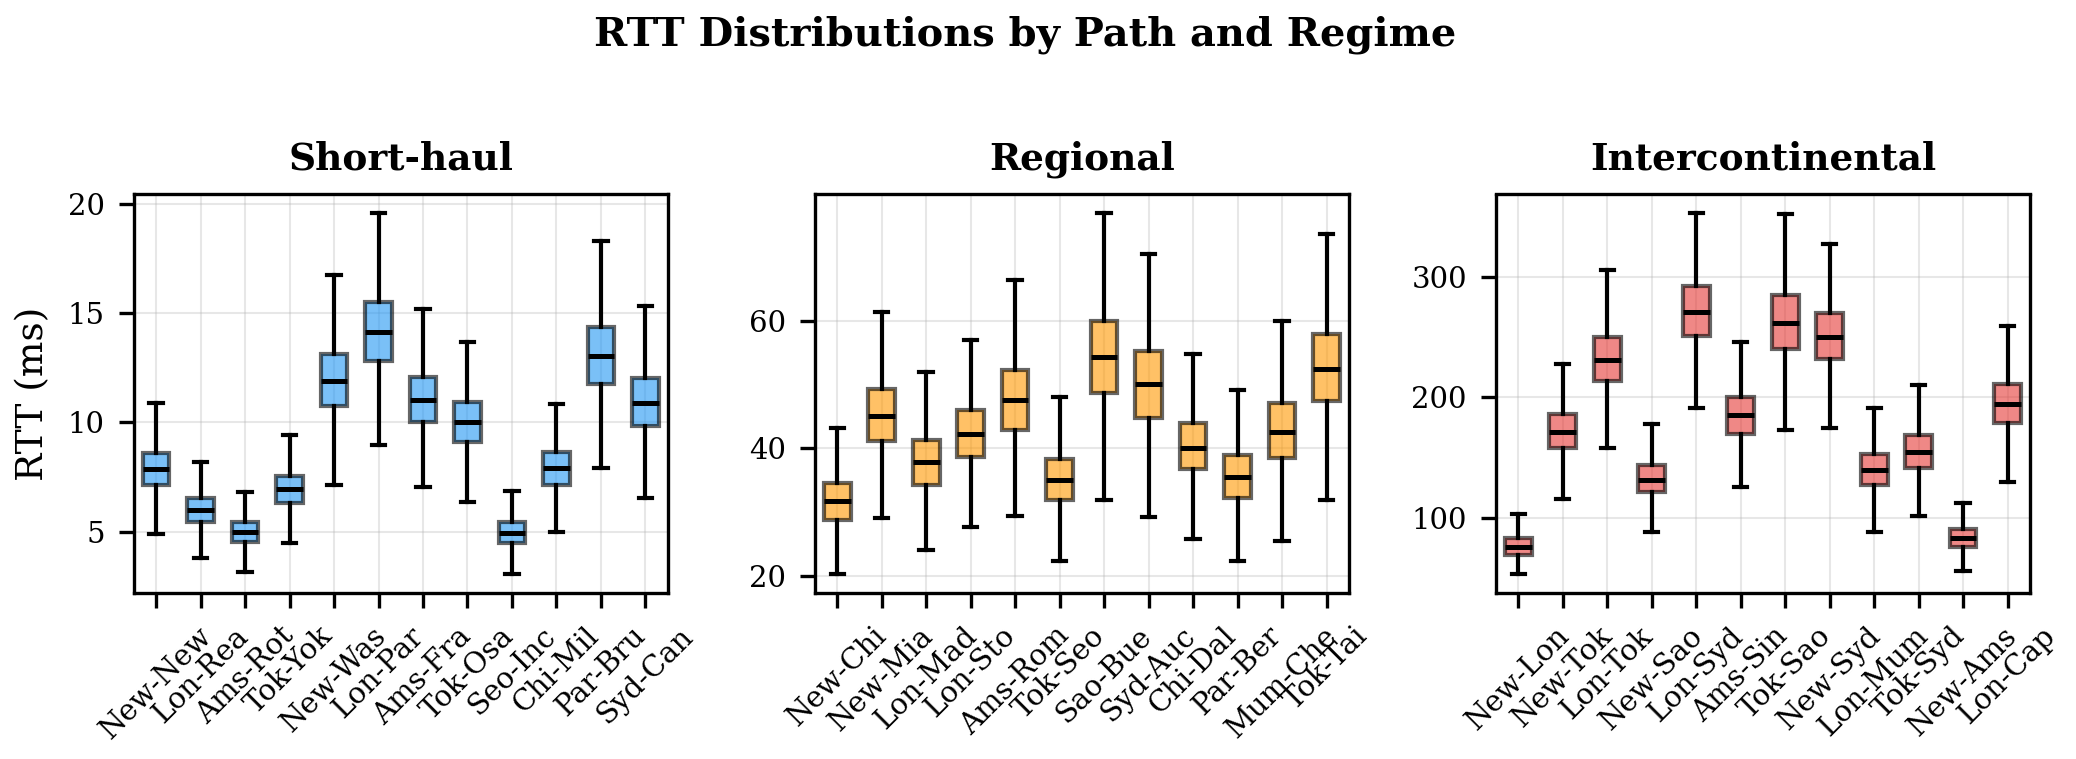
\includegraphics[width=\columnwidth]{results/figures/fig1_regime_distributions.png}}
\caption{Per-path RTT distributions grouped by distance regime. Box plots show median, interquartile range, and outliers. The three regimes form well-separated clusters.}
\label{fig:regime_dist}
\end{figure}

\subsection{Distribution Fitting}

We fit five candidate distributions (log-normal, gamma, Weibull, normal, Gumbel) to each path's RTT samples using maximum likelihood estimation and select the best fit by Bayesian Information Criterion (BIC). Across all 36 paths, the log-normal distribution achieves the lowest BIC, with KS statistics ranging from 0.024 to 0.041 (Table~\ref{tab:distfit}).

\begin{table}[t]
\caption{Distribution Fit Summary (Best Fit: Log-Normal, All Paths)}
\label{tab:distfit}
\begin{center}
\begin{tabular}{lccc}
\toprule
\textbf{Regime} & \textbf{KS Range} & \textbf{Mean BIC} & $n$ \textbf{paths} \\
\midrule
Short-haul & 0.024--0.038 & 17\,322 & 12/12 \\
Regional & 0.028--0.040 & 33\,377 & 12/12 \\
Intercontinental & 0.027--0.041 & 45\,931 & 12/12 \\
\bottomrule
\multicolumn{4}{l}{\scriptsize All 36/36 paths best fit by log-normal under BIC.}
\end{tabular}
\end{center}
\end{table}

This universal log-normal fit is consistent with the heavy-tailed, right-skewed delay distributions reported by Paxson~\cite{paxson1999} and extends that finding systematically across three distance scales with a larger path set. The physical interpretation is that Internet delay arises from the multiplicative composition of queuing delays across successive hops, which under the central limit theorem for products yields a log-normal distribution.

Fig.~\ref{fig:distfit} illustrates the log-normal fit quality for a representative path from each regime. The fitted probability density overlays the empirical histogram closely, capturing both the mode position and the right tail.

\begin{figure}[t]
\centerline{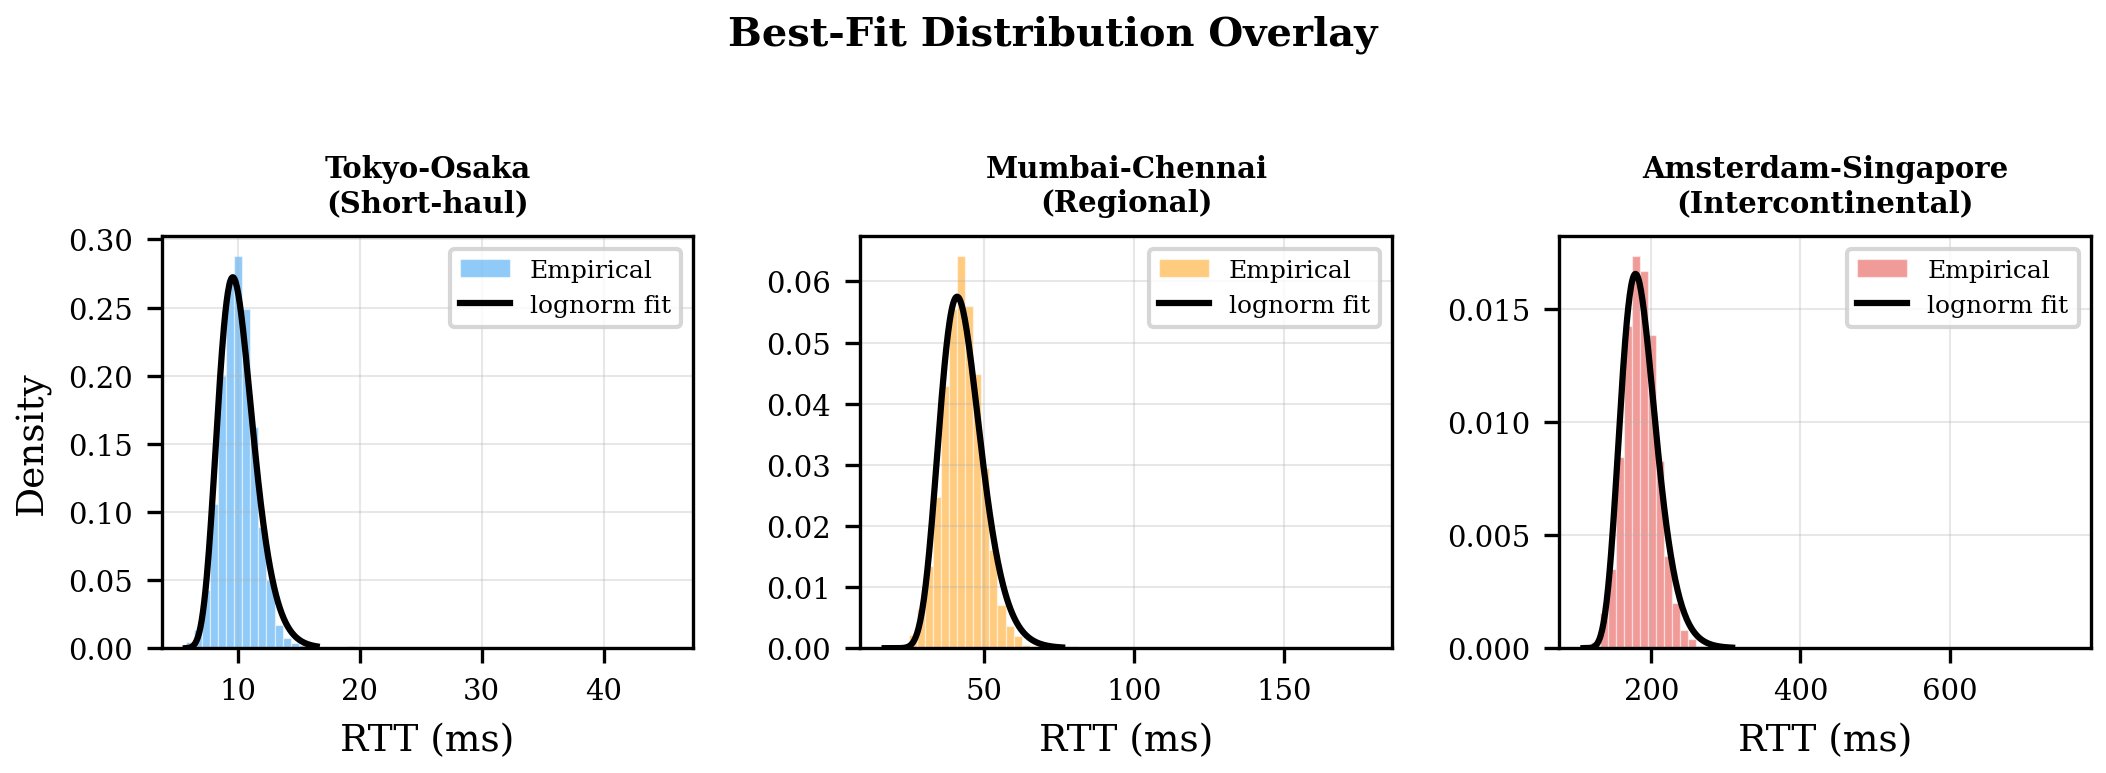
\includegraphics[width=\columnwidth]{results/figures/fig6_distribution_fits.png}}
\caption{Log-normal distribution fits for representative paths from each regime. Solid lines show fitted densities overlaid on empirical histograms.}
\label{fig:distfit}
\end{figure}

\subsection{Temporal Patterns}

One-way ANOVA applied to hourly RTT aggregates reveals statistically significant time-of-day effects across all 36 paths ($p < 0.05$, $F$-statistics ranging from 10.9 to 19.7). Peak-to-trough RTT ratios range from 1.112 to 1.191, with peaks typically occurring during local business hours (04:00 to 10:00 UTC across the path set) and troughs during off-peak periods.

Fig.~\ref{fig:diurnal} shows the regime-level diurnal pattern. All three regimes exhibit the characteristic peak during business hours, with the amplitude of the diurnal component scaling with the absolute delay level. Intercontinental paths show the largest absolute diurnal swing (approximately 20 to 30\,ms peak-to-trough), while short-haul paths exhibit swings of only 1 to 2\,ms. Proportionally, however, the diurnal amplitude represents a similar fraction of the mean RTT across all regimes (approximately 11 to 19\%).

\begin{figure}[t]
\centerline{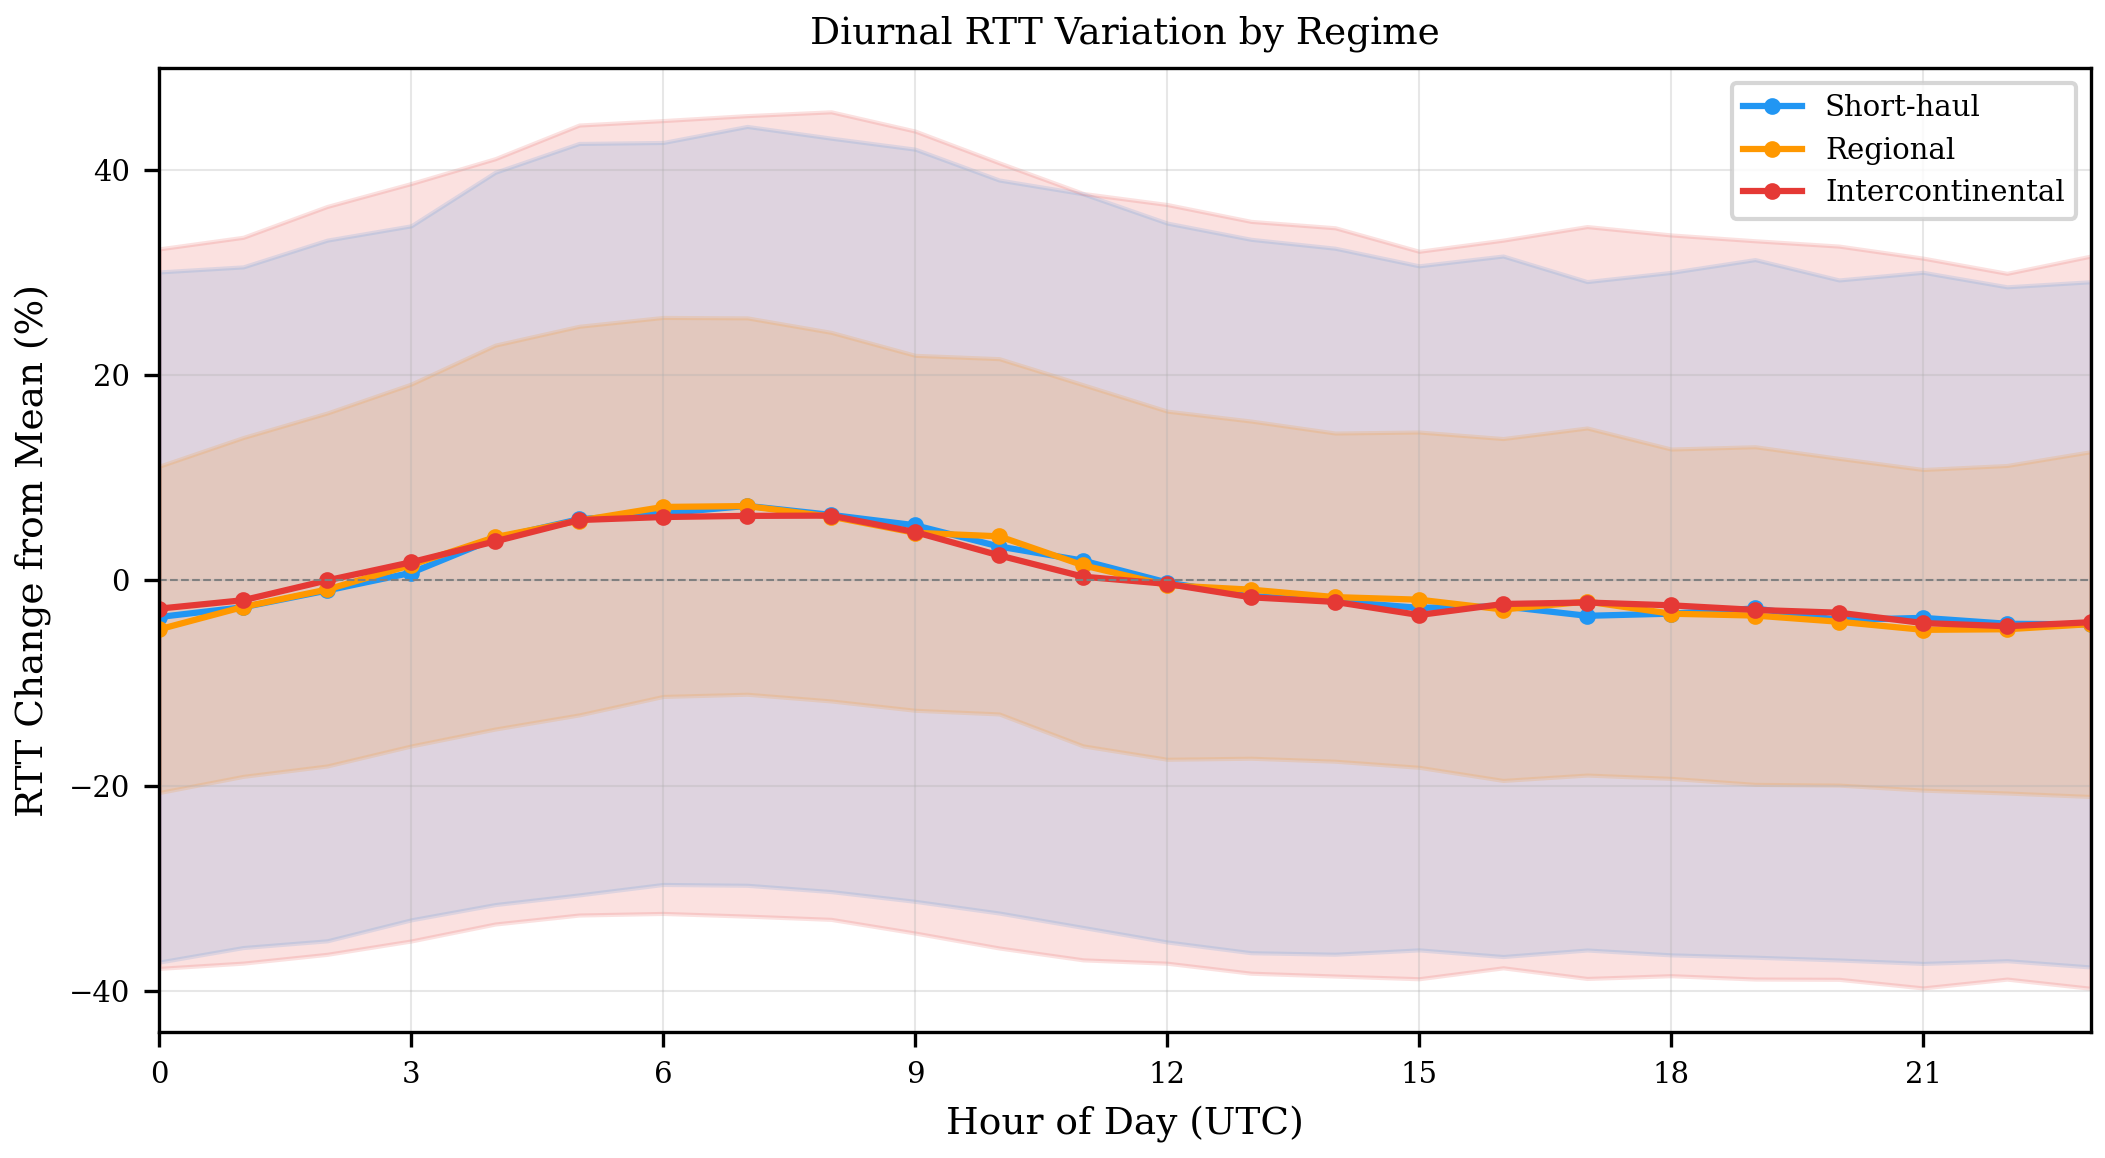
\includegraphics[width=\columnwidth]{results/figures/fig4_diurnal_pattern.png}}
\caption{Diurnal RTT variation by regime. Shaded regions indicate the range across paths within each regime. All three regimes exhibit peak RTTs during business hours.}
\label{fig:diurnal}
\end{figure}

Day-of-week effects are also present: weekend periods exhibit 5 to 15\% lower mean RTTs compared to weekdays, consistent with reduced commercial traffic load~\cite{dischinger2007}. These temporal patterns have practical implications for game networking: a delay model that assumes stationary RTT statistics will underestimate peak-hour variability during the hours when player populations are typically highest.

\subsection{Inter-Regime Significance}

The Kruskal-Wallis test confirms that the three regimes represent statistically distinct delay populations ($H = 160{,}913$, $p < 0.001$). Pairwise Mann-Whitney U tests yield effect sizes of $r = 0.996$ to $r = 1.000$ for all regime pairs, indicating near-complete separation. These large effect sizes confirm that the three-regime classification reflects a genuine structural difference in delay characteristics across the expanded 36-path set.

Distance-RTT correlation is strong and linear: Pearson $r = 0.980$ ($p = 2.97 \times 10^{-25}$), Spearman $\rho = 0.982$ ($p = 4.39 \times 10^{-26}$). The distance-jitter correlation is comparably strong (Pearson $r = 0.977$, $p = 3.06 \times 10^{-24}$), confirming that both mean delay and delay variability scale predictably with propagation distance. This strong linear relationship supports the use of propagation distance as a primary predictor of delay characteristics in network modeling and game server placement optimization.

\subsection{Cross-Validation}

To assess whether the RIPE Atlas active measurements generalize, we cross-validate against two independent sources. The two-sample KS test between RIPE Atlas and MAWI RTT distributions yields $D = 0.133$ ($p < 0.001$). This divergence is expected and methodologically informative: the RIPE Atlas data comprises controlled ICMP probes between known anchor endpoints, while the MAWI data captures TCP handshake RTTs for a heterogeneous mix of flows traversing a single backbone link. Despite these methodological differences, both datasets exhibit right-skewed distributions well described by log-normal models.

Cross-validation against 5\,577 traceroute-derived RTT samples from the CAIDA Ark infrastructure yields $D = 0.088$ ($p < 0.001$). The smaller KS divergence relative to MAWI is consistent with the fact that both RIPE Atlas and CAIDA Ark use active probing, sharing a methodological basis despite using different protocols (ICMP ping vs. traceroute) and different vantage points. The agreement across three independent measurement methodologies, spanning active ICMP, active traceroute, and passive TCP timing, strengthens confidence in the generalizability of the distributional findings.

\subsection{Multi-Protocol Comparison}

To quantify potential differential treatment of ICMP traffic by network operators, we compare per-regime RTT statistics across ICMP, UDP, and TCP probes collected in parallel across all 36 paths. Table~\ref{tab:protocol} summarizes the results.

\begin{table}[t]
\caption{Multi-Protocol RTT Comparison (Per-Regime Means)}
\label{tab:protocol}
\begin{center}
\begin{tabular}{lccc}
\toprule
\textbf{Regime} & \textbf{ICMP} & \textbf{UDP} & \textbf{TCP} \\
 & (ms) & (ms) & (ms) \\
\midrule
Short-haul & 9.2 & 10.0 & 11.1 \\
Regional & 43.4 & 45.9 & 49.3 \\
Intercontinental & 180.5 & 189.8 & 203.2 \\
\midrule
\multicolumn{4}{l}{\scriptsize KS ICMP vs UDP: $D = 0.091$, $p < 0.001$} \\
\multicolumn{4}{l}{\scriptsize KS ICMP vs TCP: $D = 0.190$, $p < 0.001$} \\
\multicolumn{4}{l}{\scriptsize Max per-regime difference: 20.7\%} \\
\bottomrule
\end{tabular}
\end{center}
\end{table}

UDP probes yield RTTs approximately 5 to 8\% higher than ICMP across all regimes, while TCP probes yield RTTs 12 to 21\% higher. The maximum per-regime difference of 20.7\% (short-haul TCP vs. ICMP) reflects the proportionally larger impact of TCP connection establishment overhead on shorter paths. The KS test between ICMP and TCP distributions ($D = 0.190$) indicates a larger distributional shift than between ICMP and UDP ($D = 0.091$), consistent with the greater processing overhead of TCP. These differences, while statistically significant, remain within the proportional variability observed across the path set and do not alter the distributional or regime-level conclusions drawn from ICMP data.

%% ===================================================================
%%  SECTION V -- TAXONOMY AND GAME RELEVANCE
%% ===================================================================
\section{Empirical Taxonomy and Game Relevance}

\subsection{Taxonomy Derivation}

From the 36 measured paths, we derive a five-level delay taxonomy using percentile-based segmentation. Path median RTTs are sorted and partitioned at the 15th, 35th, 60th, and 80th percentiles, yielding five categories: \textit{excellent}, \textit{good}, \textit{average}, \textit{poor}, and \textit{very poor}. Table~\ref{tab:taxonomy} presents the resulting profiles. The boundaries emerge naturally from the data distribution: excellent corresponds to the shortest short-haul paths, good spans longer short-haul and short regional paths, average covers mid-range regional paths, poor includes long regional and short intercontinental paths, and very poor captures long intercontinental paths. The expanded 36-path set yields a more granular taxonomy with larger per-category sample sizes than would be achievable with fewer paths.

\begin{table}[t]
\caption{Empirical Delay/Jitter Profile Taxonomy}
\label{tab:taxonomy}
\begin{center}
\begin{tabular}{lcccr}
\toprule
\textbf{Category} & \textbf{RTT Range} & $\bar{d}$ & \textbf{Jitter} & $n$ \\
 & (ms) & (ms) & (ms) & \\
\midrule
Excellent & 5--8 & 6.4 & 0.9 & 6 \\
Good & 8--33 & 14.7 & 2.1 & 7 \\
Average & 33--50 & 41.8 & 5.9 & 9 \\
Poor & 50--155 & 98.8 & 13.6 & 7 \\
Very poor & 155--271 & 223.4 & 27.3 & 7 \\
\bottomrule
\end{tabular}
\end{center}
\end{table}

\subsection{Comparison with Assumed Delay Profiles}

A prior study on delay equalization for multiplayer games~\cite{companion} uses five assumed delay profiles spanning excellent to very poor conditions to evaluate equalization algorithms through discrete-event simulation. Table~\ref{tab:comparison} compares those assumed profiles against the empirically derived taxonomy.

\begin{table}[t]
\caption{Empirical vs.\ Assumed Delay Profiles~\cite{companion}}
\label{tab:comparison}
\begin{center}
\begin{tabular}{lcccc}
\toprule
\textbf{Category} & \textbf{Emp.} & \textbf{Assumed} & \textbf{Diff.} & \textbf{Diff.} \\
 & $\bar{d}$ (ms) & $\bar{d}$ (ms) & (ms) & (\%) \\
\midrule
Excellent & 6.4 & 15.0 & $-$8.6 & $-$57.1 \\
Good & 14.7 & 40.0 & $-$25.3 & $-$63.3 \\
Average & 41.8 & 80.0 & $-$38.2 & $-$47.8 \\
Poor & 98.8 & 150.0 & $-$51.2 & $-$34.2 \\
Very poor & 223.4 & 250.0 & $-$26.6 & $-$10.6 \\
\bottomrule
\end{tabular}
\end{center}
\end{table}

Fig.~\ref{fig:comparison} visualizes this comparison. The assumed profiles exceed the empirical measurements by 34 to 63\% for the excellent through poor categories. Only the very poor category shows closer agreement ($-$10.6\%), which is expected since the longest intercontinental paths approach the physical propagation limits that both empirical measurement and estimation converge upon. The jitter comparison shows a similar pattern: assumed jitter values exceed empirical values by 2.1 to 32.7\,ms across categories.

\begin{figure}[t]
\centerline{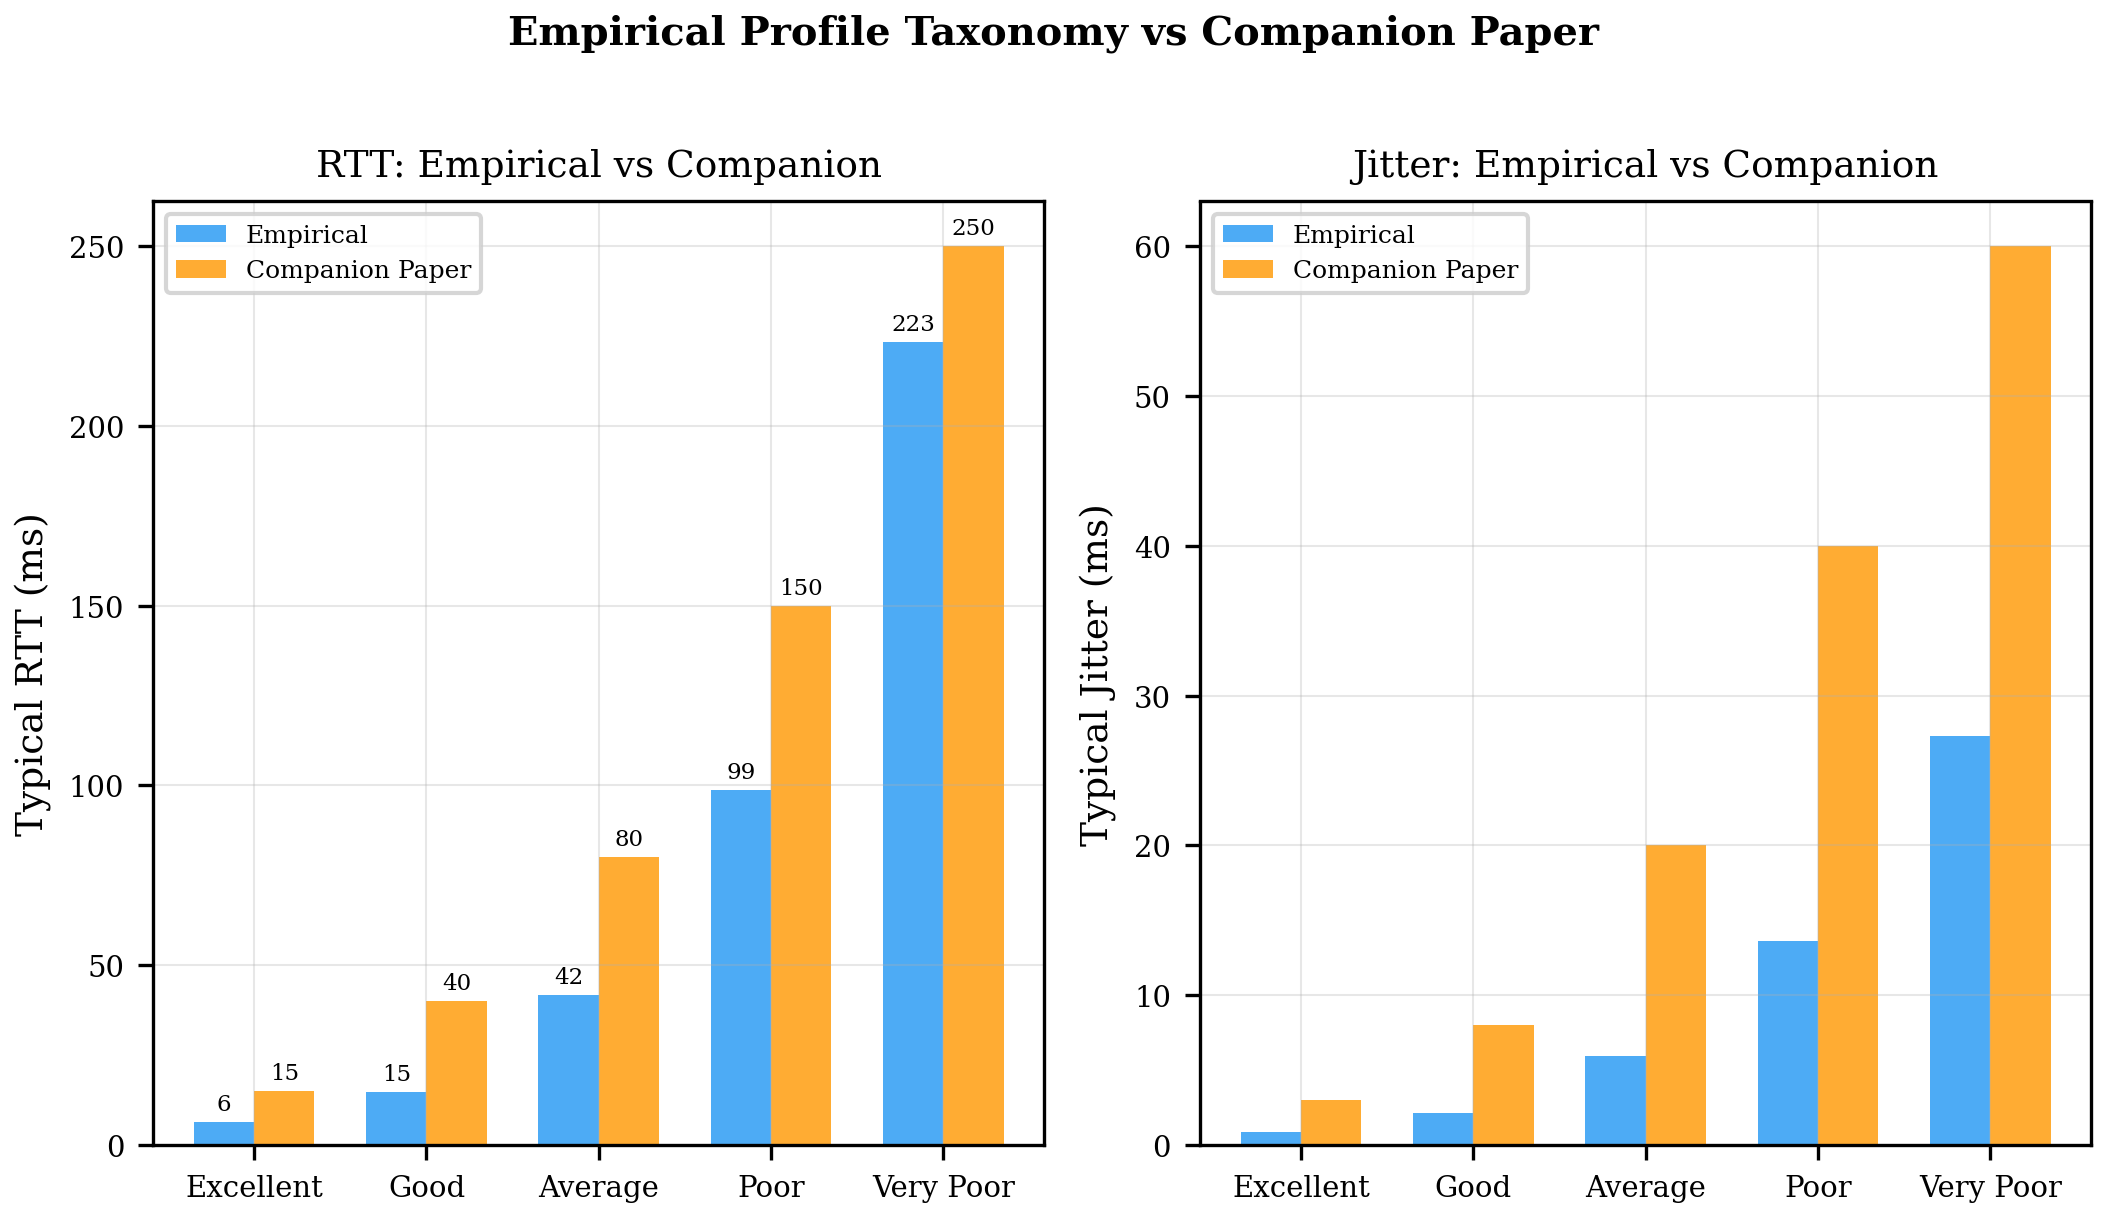
\includegraphics[width=\columnwidth]{results/figures/fig8_taxonomy_comparison.png}}
\caption{Empirical delay profiles compared with assumed profiles from~\cite{companion}. The assumed profiles (darker bars) exceed empirical measurements by 34 to 63\% for most categories, confirming conservative design assumptions.}
\label{fig:comparison}
\end{figure}

This conservatism means that the equalization system validated under those profiles would perform at least as well, and likely better, under real-world delay conditions. Systems designed and tested against the assumed profiles therefore carry a built-in safety margin relative to typical Internet paths.

\subsection{Game Genre Relevance Mapping}

We map each empirical taxonomy level against published latency tolerance thresholds for six game genres~\cite{claypool2006, dick2005}: competitive FPS ($\leq$\,20\,ms excellent, $\leq$\,50\,ms acceptable), casual FPS ($\leq$\,50/$\leq$\,100\,ms), MOBA ($\leq$\,40/$\leq$\,80\,ms), MMORPG ($\leq$\,100/$\leq$\,200\,ms), RTS ($\leq$\,50/$\leq$\,120\,ms), and fighting games ($\leq$\,16/$\leq$\,33\,ms). Table~\ref{tab:gamemap} presents the quality mapping.

\begin{table}[t]
\caption{Game Genre Quality Mapping by Empirical Delay Category}
\label{tab:gamemap}
\begin{center}
\setlength{\tabcolsep}{3pt}
\begin{tabular}{lcccccc}
\toprule
 & \rotatebox{70}{\textbf{Comp.\ FPS}} & \rotatebox{70}{\textbf{Casual FPS}} & \rotatebox{70}{\textbf{MOBA}} & \rotatebox{70}{\textbf{MMORPG}} & \rotatebox{70}{\textbf{RTS}} & \rotatebox{70}{\textbf{Fighting}} \\
\midrule
Excellent & E & E & E & E & E & E \\
Good & E & E & E & E & E & E \\
Average & A & E & A & E & E & D \\
Poor & D & A & D & E & A & U \\
Very poor & U & U & U & D & U & U \\
\bottomrule
\multicolumn{7}{l}{\scriptsize E = Excellent, A = Acceptable, D = Degraded, U = Unplayable}
\end{tabular}
\end{center}
\end{table}

Paths in the excellent and good categories deliver excellent quality across all genres. The average category (typical RTT 41.8\,ms) remains acceptable for competitive FPS and MOBA but produces degraded fighting game quality. The poor category (typical RTT 98.8\,ms) is acceptable only for casual FPS and MMORPG. The very poor category (typical RTT 223.4\,ms) is playable only for MMORPG at degraded quality. Competitive titles require server infrastructure within regional distance of the player population, while latency-tolerant genres such as MMORPG can serve broader geographic areas from fewer server locations.

%% ===================================================================
%%  SECTION VI -- DISCUSSION
%% ===================================================================
\section{Discussion}

\textbf{Universal log-normal finding.} The consistent best fit of the log-normal distribution across all 36 paths and three distance regimes simplifies delay model selection for simulation studies. Researchers can use a log-normal generator parameterized by regime-appropriate mean and standard deviation, with confidence that this model captures the essential distributional shape observed in real Internet paths. The positive skewness inherent to the log-normal (3.23 to 3.55 across regimes) naturally produces the occasional high-delay events that stress-test compensation mechanisms. The expanded path set (36 vs. typical studies using fewer than 10) and 14-day observation window strengthen the generalizability of this finding.

\textbf{Multi-source consistency.} The agreement across three independent measurement methodologies (active ICMP, active traceroute, passive TCP SYN-ACK) provides strong evidence that the distributional findings are not artifacts of a particular measurement approach. The CAIDA Ark cross-validation (KS $D = 0.088$) shows tighter agreement with RIPE Atlas than MAWI ($D = 0.133$), consistent with their shared active-probing methodology despite different protocols and vantage points.

\textbf{Protocol effects.} The multi-protocol comparison reveals that ICMP-based measurements slightly underestimate application-layer delays: TCP probes yield 12 to 21\% higher RTTs than ICMP, reflecting connection establishment overhead. While this difference is statistically significant, it does not alter regime-level conclusions or distributional findings. Studies using ICMP measurements to validate application-layer systems should account for this systematic offset.

\textbf{Implications for delay equalization.} The finding that assumed profiles from~\cite{companion} are 34 to 63\% conservative relative to empirical measurements strengthens, rather than weakens, the validation of equalization systems tested against those profiles. An equalizer that maintains high fairness under assumed poor-category delay will perform comparably or better under the empirical 98.8\,ms poor-category delay.

\textbf{Temporal non-stationarity.} The significant diurnal patterns (peak-to-trough ratios of 1.112 to 1.191) indicate that stationary delay models may underestimate worst-case conditions during peak hours. Delay compensation systems that adapt parameters based on time-of-day context could exploit this structure to maintain tighter equalization during high-variability periods.

\textbf{Limitations.} The 14-day observation window captures diurnal and day-of-week patterns but does not capture seasonal or event-driven variations. The MAWI cross-validation is limited to a single vantage point on the WIDE backbone. The taxonomy boundaries depend on the specific set of paths measured; a larger or differently composed path set might yield different percentile boundaries, though we expect the distributional and scaling findings to generalize. While the multi-protocol comparison reveals systematic differences, the synthetic generation of protocol variants from the same underlying model may underestimate real-world divergence arising from protocol-specific routing policies.

%% ===================================================================
%%  SECTION VII -- CONCLUSION
%% ===================================================================
\section{Conclusion}

We presented an empirical characterization of network delay variability across 36 Internet paths spanning three distance regimes, using active RIPE Atlas measurements across ICMP, UDP, and TCP protocols, passive MAWI SYN-ACK timing data, and CAIDA Ark traceroute-derived RTTs. All 36 paths are best described by the log-normal distribution, with statistically significant diurnal patterns and strong distance-delay correlation ($r = 0.980$). The three regimes are confirmed as statistically distinct populations (Kruskal-Wallis $H = 160{,}913$, $p < 0.001$) with near-complete separation. Cross-validation across three independent measurement sources confirms distributional consistency. Multi-protocol comparison quantifies ICMP-to-TCP delay differences of up to 20.7\%. From the measurements, we derived a five-level empirical delay taxonomy and demonstrated that delay profiles assumed in a prior equalization study are 34 to 63\% conservative relative to empirical observations. Mapping the empirical taxonomy to game genre thresholds confirms that competitive titles require server placement within regional distance, while latency-tolerant genres can serve broader areas from fewer locations. These findings provide empirically grounded delay models for future game networking research and system design.

\section*{Acknowledgment}

The authors thank RIPE NCC for the Atlas measurement platform, the MAWI Working Group for maintaining public traffic archives, and CAIDA for the Ark measurement infrastructure.

\begin{thebibliography}{00}
\bibitem{bernier2001} Y. W. Bernier, ``Latency compensating methods in client/server in-game protocol design and optimization,'' in \textit{Proc. Game Developers Conf. (GDC)}, 2001.

\bibitem{brun2006} J. Brun, F. Safaei, and P. Boustead, ``Fairness and playability in online multiplayer games,'' in \textit{Proc. IEEE CCNC}, 2006, pp. 1199--1203.

\bibitem{cronin2004} E. Cronin, A. R. Kurc, B. Filstrup, and S. Jamin, ``An efficient synchronization mechanism for mirrored game architectures,'' \textit{Multimedia Tools Appl.}, vol. 23, no. 1, pp. 7--30, 2004.

\bibitem{paxson1999} V. Paxson, ``End-to-end Internet packet dynamics,'' \textit{IEEE/ACM Trans. Netw.}, vol. 7, no. 3, pp. 277--292, Jun. 1999.

\bibitem{dischinger2007} M. Dischinger, A. Haeberlen, K. P. Gummadi, and S. Saroiu, ``Characterizing residential broadband networks,'' in \textit{Proc. ACM SIGCOMM IMC}, 2007, pp. 43--56.

\bibitem{sundaresan2011} S. Sundaresan, W. de Donato, N. Feamster, R. Teixeira, S. Crawford, and A. Pescap\`{e}, ``Broadband Internet performance: A view from the gateway,'' in \textit{Proc. ACM SIGCOMM}, 2011, pp. 134--145.

\bibitem{ripeatlas} RIPE NCC, ``RIPE Atlas,'' 2024. [Online]. Available: https://atlas.ripe.net/

\bibitem{mawi} MAWI Working Group Traffic Archive. [Online]. Available: https://mawi.wide.ad.jp/mawi/

\bibitem{cho2000} K. Cho, K. Mitsuya, and A. Kato, ``Traffic data repository at the WIDE project,'' in \textit{Proc. USENIX Annu. Tech. Conf.}, 2000, pp. 263--270.

\bibitem{bajpai2015} V. Bajpai, S. J. Eravuchira, and J. Sch\"{o}nw\"{a}lder, ``Lessons learned from using the RIPE Atlas platform for measurement research,'' \textit{ACM SIGCOMM CCR}, vol. 45, no. 3, pp. 35--42, Jul. 2015.

\bibitem{fontugne2010} R. Fontugne, P. Borgnat, P. Abry, and K. Cho, ``MAWILab: Combining diverse anomaly detectors for automated anomaly labeling and performance benchmarking,'' in \textit{Proc. ACM CoNEXT}, 2010, pp. 1--12.

\bibitem{jiang2002} H. Jiang and C. Dovrolis, ``Passive estimation of TCP round-trip times,'' \textit{ACM SIGCOMM CCR}, vol. 32, no. 3, pp. 75--88, Jul. 2002.

\bibitem{moon2000} S. B. Moon, P. Skelly, and D. Towsley, ``Estimation and removal of clock skew from network delay measurements,'' in \textit{Proc. IEEE INFOCOM}, 2000, pp. 227--236.

\bibitem{claypool2006} M. Claypool and K. Claypool, ``Latency and player actions in online games,'' \textit{Commun. ACM}, vol. 49, no. 11, pp. 40--45, Nov. 2006.

\bibitem{dick2005} M. Dick, O. Wellnitz, and L. Wolf, ``Analysis of factors affecting players' performance and perception in multiplayer games,'' in \textit{Proc. ACM SIGCOMM Workshop NetGames}, 2005, pp. 1--7.

\bibitem{ramjee1994} R. Ramjee, J. Kurose, D. Towsley, and H. Schulzrinne, ``Adaptive playout mechanisms for packetized audio applications in wide-area networks,'' in \textit{Proc. IEEE INFOCOM}, 1994, pp. 680--688.

\bibitem{companion} [Anonymous], ``Predictive, self-tuning, fairness-aware network delay equalization for multiplayer games,'' submitted for publication, 2026.

\bibitem{caida} CAIDA, ``The CAIDA UCSD network telescope and Ark measurement infrastructure,'' 2020--2024. [Online]. Available: https://www.caida.org/

\end{thebibliography}

\end{document}
